
\chapter{Description de l'API de \PpFf}
\label{description.chap}



\begin{figure}[H]
\centering
     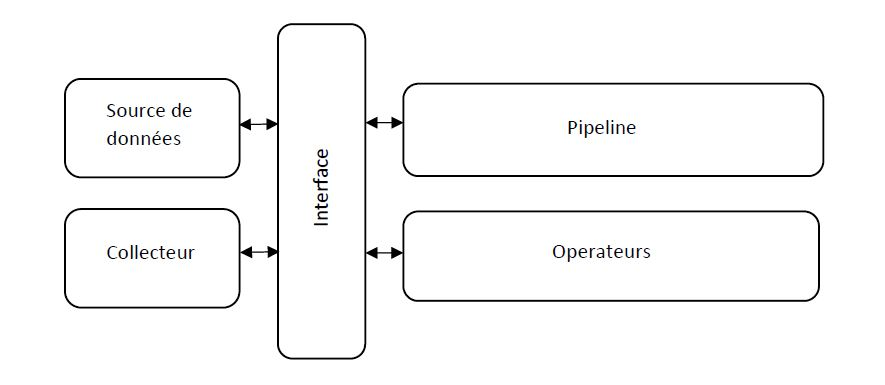
\includegraphics[ height=15cm, width=9cm]{Figures/ComponentsAPI.jpg}
      \caption{Les m\'ethodes expos\'ees par l'{API} group\'ees par leur fonctionnalit\'e.}
       \label{ClassDiagramme.fig}
\end{figure}



Ce chapitre pr\'esente l'API de \ppff. Sa conception permet aux utilisateurs de tirer parti de la simplicit\'e d'utilisation tout en cachant la complexit\'e concernant les m\'ecanismes concurrents utilis\'es. La figure~\ref{ComponentsAPI.fig} pr\'esente une vue d'ensemble des principaux \'el\'ements de \ppff. Bas\'e sur la fonctionnalit\'e l'API --- l'interface avec laquelle interagit le d\'eveloppeur --- est divis\'ee en trois cat\'egories : les \TT{Source}s, les \TT{Transformation}s et les \TT{Colector}s. 
Le r\^ole de chaque cat\'egorie dans l'API est pr\'esent\'e dans les sections suivante. Le chapitre pr\'esente \'egalement le code source d'un petit exemple, \TT{WordCount}, pour illustrer l'utilisation de l'API et l'effet des principales op\'erations.

L'{API} de \PpFf{} est impl\'ement\'ee au-dessus de la biblioth\`eque \TT{FastFlow}, impl\'ementation qui sera d\'ecrite au prochain chapitre.



\section{L'application WordCount}

\begin{lstlisting}[
label={wordcount.c++},
language=c++,
caption={Le code source d'une application pour compter le nombre d'occurrences de mots dans un texte.},
frame=single,
float]
typedef std::vector<std::string> Words;

bool notEmpty(std::string* s) { return s->size() > 0; }

int main(int argc, char* argv[]) {
  Reducer<std::string, int> sumOccurrences(
    0, 
    [](int count, std::string _) { return count + 1; },
    std::plus<int>{} );

  std::string path = "/home/Words.txt"; 

  std::unordered_map<std::string, int> currentResult = 
	Pipe()
    .linesFromFile(path) 
    .parallel(4)
    .flatMap<std::string, std::string, Words>(splitInWords)
    .map<std::string, std::string>(toLowercaseLetters)
    .find<std::string>(notEmpty)
    .reduceByKey<std::string, std::string, int>(sumOccurrences);
}
\end{lstlisting}

L'application \TT{WordCount} pr\'esent\'ee dans ce chapitre illustre le fonctionnement de \TT{PpFf}. Le code source est montr\'e dans le listing~\ref{wordcount.c++}. L'application compte le nombre d'occurrences des mots dans un fichier texte. Une telle application est compos\'ee de plusieurs \'etapes. 

La premi\`ere \'etape d\'efinit la source du flux. Dans l'application de compte de mots, la source est constitu\'ee par les lignes contenues dans un fichier. C'est la m\'ethode \TT{linesFromFile(path)} qui permet d'extraire et retourner dans le flux les lignes du fichier. Le fichier est sp\'ecifi\'e par la variable \TT{path} fournie en argument \`a la m\'ethode \TT{linesFromFile}. 

Dans notre exemple, la deuxi\`eme \'etape dans l'application de compte de mots est l'appel \`a \TT{parallel}. Ceci permet de partitionner les \'el\'ements du flux entre divers \emph{threads} --- ici, quatre (4) \emph{threads} --- et donc d'ex\'ecuter les \'etapes qui suivent en parall\`ele. 

Les op\'erations subs\'equentes du pipeline sont les suivantes :
\begin{itemize}

\item L'op\'eration \TT{flatMap} d\'ecompose chaque ligne en mots individuels en appliquant la fonction \TT{splitInWords} sur chacune des lignes;

\item L'op\'eration \TT{map} transforme chacun des mots en rempla\c{c}ant les lettres majuscules d'un mot en lettres minuscules en appliquant la fonction \TT{toLowerCaseLetters}.

\item L'op\'eration \TT{find} retourne dans le flux seulement les mots qui ne sont pas vides (\TT{notEmpty}).

\item Finalement, l'op\'eration \TT{reduceByKey}  regroupe les mots similaires ensemble et compte le nombre d'occurrences de chaque mot, et ce par l'utilisation du \TT{Reducer} \TT{sumOccurrences}. 
\end{itemize}


\section{Les flux de donn\'ees: type \TT{Flow}}

L'interface propos\'ee en \TT{PpFf} consiste en un ensemble de m\'ethodes qui permettent \`a l'utilisateur de manipuler des flux de donn\'ees de mani\`ere simple et efficace. L'interface suit d'assez pr\`e celle introduite pour les Streams de Java 8. Le tableau~\ref{methodes_api.tab} d\'ecrit bri\`evement les m\'ethodes --- group\'es par leurs fonctionnalit\'es --- export\'ees par l'API.


%\begin{landscape}
\newpage
\KOMAoptions{paper=landscape,pagesize}
\recalctypearea


\begin{center}
\footnotesize
\begin{longtable}{|l|l|p{5cm}|}
\caption{Les m\'ethodes publiques de l'API de~\ppff.\label{methodes_api.tab}}\\
\hline
\textbf{M\'ethode} & \textbf{Type du r\'esultat} & \textbf{Description du r\'esultat}\\
\hline
\endfirsthead
\multicolumn{3}{c}%
{\tablename\ \thetable\ Méthodes publiques de l'API (\textit{suite})} \\
\hline
\textbf{M\'ethode} & \textbf{Type du r\'esultat} & \textbf{Description du r\'esultat}\\
\hline
\endhead
\hline \multicolumn{3}{r}{\textit{Suite page suivante}} \\
\endfoot
\hline
\endlastfoot
\hline
	\multicolumn{3}{|c|}{Source --- M\'ethodes pour g\'en\'erer un nouveau flux \`a partir d'une source}
    \\
\hline
	\begin{tabular}{@{}l@{}}
	\tt linesFromFile(string\& path)
	\end{tabular} &
	\TT{Flux\&} & 
    Retourne un flux avec les lignes
    contenues dans le fichier indiqu\'e par \TT{path}.
    \\
\hline
	\begin{tabular}{@{}l@{}}
	\tt template<T, Iterator> \\
	\tt source(Iterator  begin, Iterator end)
	\end{tabular} &
	\TT{Flux\&} &
	Convertit un conteneur de type {STL} en flux.
    \\
\hline
	\multicolumn{3}{|c|}{Transformation --- M\'ethodes pour produire un flux \`a partir d'un flux existant}
    \\    
\hline
	\begin{tabular}{@{}l@{}}
	\tt template<In> \\
	\tt find(Func<bool(In*)> const\& predicate)
	\end{tabular} &
  	\TT{Flux\&} &
    Retourne les
    \'el\'ements du flux qui satisfont \TT{predicate}.
    \\
\hline
	\begin{tabular}{@{}l@{}}
	\tt template<In, Out, Container> \\
	\tt flatMap(Func<Container*(In*)> const\& taskFunc)
	\end{tabular} &
  	\TT{Flux\&} & 
    Applique la fonction fournie en argument
    \`a chaque \'el\'ement du flux et concat\`ene ces \'el\'ements lorsque plusieurs sont produits par la fonction.
    \\
\hline
	\begin{tabular}{@{}l@{}}
	\tt template<In, Out, Container=In> \\
	\tt flatMap()
	\end{tabular} &
  	\TT{Flux\&} &
    Produit un flux avec les \'el\'ements du conteneur.  
    \\
\hline
	\begin{tabular}{@{}l@{}}
	\tt template<T> \\
	\tt limit(int n)
	\end{tabular} &
	\TT{Flux\&} & 
    Retourne un flux compos\'e des \TT{n}~premiers \'el\'ements du flux d'entr\'ee.
    \\
\hline
	\begin{tabular}{@{}l@{}}
	\tt template<In, Out> \\
	\tt map(Func<Out*(In*)> const\& taskFunc)
	\end{tabular} &
	\TT{Flux\&} & 
    Retourne un flux compos\'e de
    l'application de \TT{taskFunc}
    \`a chacun des
    \'el\'ements du flux.
    \\
\hline
	\begin{tabular}{@{}l@{}}
	\tt template<In> \\
	\tt peek(Func<void(In*)> const\& taskFunc)
	\end{tabular} &
	\TT{Flux\&} &
	Applique la fonction \TT{taskFunc} \`a chaque \'el\'ement du flux et r\'e\'emet l'\'el\'ement (sans le modifier) sur le flux de sortie. Note: Utile pour le d\'ebogage.
    \\
\hline
	\begin{tabular}{@{}l@{}}
	\tt template<T> \\
	\tt skip(int n)
	\end{tabular} &
	\TT{Flux\&} &
    Retourne un flux compos\'e des \'el\'ements du flux d'entr\'ee, mais en omettant les \TT{n} premiers \'el\'ements.
    \\
\hline
	\multicolumn{3}{|c|}{Collector --- M\'ethodes qui produisent une valeur, typiquement scalaire, \`a partir d'un flux}
    \\     
\hline
	\begin{tabular}{@{}l@{}}
	\tt template<T> \\
	\tt allMatch(Func<bool(T*)> predicate)
	\end{tabular} &
  	\TT{bool} &
    Retourne \TT{true} si tous les \'el\'ements
    du flux satisfont \TT{predicate}, sinon \TT{false}.
    \\
\hline
	\begin{tabular}{@{}l@{}}
	\tt template<T> \\
	\tt anyMatch(Func<bool(T*)> predicate)
	\end{tabular} &
  	\TT{bool} & 
    Retourne \TT{true} si au moins un  
    \'el\'ement du flux satisfait \TT{predicate}, sinon \TT{false}.
\\          
\hline
	\begin{tabular}{@{}l@{}}
	\tt count()\\
	\end{tabular} &
  	\TT{unsigned int} & 
    Retourne le nombre d'\'el\'ements
    du flux.
    \\ 
\hline
	\begin{tabular}{@{}l@{}}
	\tt template<T> \\
	\tt max(Func<void(T*, T*)> compare)
	\end{tabular} &
	\TT{T} &
	Retourne l'\'el\'ement maximum du flux en fonction du comparateur.
    \\
\hline
	\begin{tabular}{@{}l@{}}
	\tt template<T> \\
	\tt min(Func<void(T*, T*)> compare)
	\end{tabular} &
	\TT{T} &
	Retourne l'\'el\'ement minimum du flux en fonction du comparateur.
    \\
\hline
	\begin{tabular}{@{}l@{}}
	\tt template<T> \\
	\tt noneMatch(Func<bool(T*)> predicate)
	\end{tabular} &
	\TT{bool} &
    Retourne \TT{true} si aucun des \'el\'ements
    du flux ne satisfait \TT{predicate},
    sinon \TT{false}.
    \\    
\hline
	\begin{tabular}{@{}l@{}}
	\tt template<In, Out=In> \\
	\tt reduce(Reducer<In, Out> const\& reducer)
	\end{tabular} &
	\TT{Out} &
	Effectue une r\'eduction sur les \'el\'ements du flux. Voir la notion de \TT{reducer}, p.~\pageref{reducer.sect}.
    \\
\hline
	\begin{tabular}{@{}l@{}}
	\tt template<In, Out=In> \\
	\tt reduce(Out init, Func<Out(In, Out)> acc)
	\end{tabular} &
	\TT{Out} &
	Effectue une r\'eduction des \'el\'ements du flux, en utilisant \TT{init} comme valeur initiale et \TT{acc} comme fonction d'accumulation.
    \\    
\hline
	\begin{tabular}{@{}l@{}}
	\tt template<T> \\
	\tt sum()
	\end{tabular} &
	\TT{T} &
	Retourne la somme des \'el\'ements du flux.
    \\
\hline
	\multicolumn{3}{|c|}{Collector --- M\'ethodes qui produisent une collection \`a partir d'un flux}
    \\     
\hline
	\begin{tabular}{@{}l@{}}
	\tt template<T, Container<T>{>}\\
	\tt collect()
	\end{tabular} &
  	\TT{Container<T>} &
    Retourne un conteneur
    STL avec tous les \'el\'ements du flux.
    \\
\hline
	\begin{tabular}{@{}l@{}}
	\tt template<In, K=In, V=In, MapType> \\
	\tt groupByKey(Func<K*(In*)> fk, Func<V*(In*)> fv)
	\end{tabular} &
  	\TT{MapType} &
    Retourne un dictionnaire (\emph{map}) avec les \'el\'ements
    du flux regroupés par cl\'e.
   \\
\hline
	\begin{tabular}{@{}l@{}}
	\tt template<In, K=In, V=In, MapType> \\
	\tt reduceByKey(Reducer<In, V> r, Func<K*(In*)> fk)
	\end{tabular} &
	\TT{MapType} &
    Effectue une r\'eduction sur les valeurs de chaque cl\'e à l'aide d'op\'erateur \TT{Reducer}. Voir la notion de \TT{Reducer}, p.~\pageref{reducer.sect}.
    \\
\hline
	\begin{tabular}{@{}l@{}}
	\tt template<T> \\
	\tt sort(Func<bool(T, T)> const\& compare)
	\end{tabular} &
	\TT{Collection<T, Container>} &
	Effectue le tri des \'el\'ements du flux, selon l'ordre sp\'ecifi\'e par \TT{compare}. Note: Le premier \'el\'ement du flux de sortie n'est \'emis \emph{qu'apr\`es que la fin de flux ait \'et\'e rencontr\'ee}.
    \\
\hline
	\multicolumn{3}{|c|}{Autre m\'ethode influen\c{c}ant le comportement du traitement du flux}
    \\      
\hline
	\begin{tabular}{@{}l@{}}
	\tt parallel(int workers = 1)
	\end{tabular} &
	\TT{Flux\&} &
	Sp\'ecifie le nombre de travailleurs \`a utiliser pour traiter les \'el\'ements du flux.
    \\    
\hline    
\end{longtable}
\normalsize
\end{center}

\newpage
\KOMAoptions{paper=portrait,pagesize}
\recalctypearea


Comme on peut le voir dans le tableau~\ref{methodes_api.tab}, la d\'eclaration des m\'ethodes utilise la programmation g\'en\'erique de C++, c'est-\`a-dire les \emph{templates}. Cela permet aux utilisateurs d'avoir une interface g\'en\'erique unique, de sorte qu'une m\'ethode peut \^etre r\'eutilis\'ee pour n'importe quel type de donn\'ees.


Un autre point cl\'e dans cette interface est son expressivit\'e. M\^eme avant sa conception d\'etaill\'ee, nous nous \'etions donn\'es comme objectif de fournir un syst\`eme suffisamment intuitif et expressif pour le traitement de flux de donn\'ees.


\begin{lstlisting}[
label={expressivite_api.c++},
language=c++,
caption={Un exemple illustrant les op\'erations de l'API de \ppff.},
frame=single,
float]
// Definition (omise) d'un vecteur d'objets Employee.
std::vector<Employee> sourceEmployees;
...

std::vector<Employee> result = 
   Pipe()
   .source<Employee>(sourceEmployees.begin(), sourceEmployees.end())
   .find<Employee>([](Employee *e) { return e->salary > 35000; })
   .collect<Employee, std::vector>();
\end{lstlisting}


Le listing~\ref{expressivite_api.c++} pr\'esente un extrait de code C++ qui donne un premier aper\c{c}u de l'expressivit\'e de l'interface --- d'autres exemples seront pr\'esent\'es plus loin. Dans cet exemple, on s\'electionne les employ\'es qui ont un salaire plus grand que 35~K\$. Les employ\'es sont initialement dans un conteneur STL et sont filtr\'es en chainant trois op\'erations : $i)$ \TT{source} qui permet d'envoyer dans le flux des objets de type~\TT{Employe}; $ii$) \TT{find} qui s\'electionne les employ\'es selon la condition fournie en param\`etre (une lambda-expression); $iii)$ \TT{collect} qui met les employ\'es s\'electionn\'es dans un conteneur STL. Ici, les employ\'es s\'electionn\'es sont mis dans un conteneur de type \TT{std::vector} --- le type de conteneur est donn\'e par le type fourni en argument (g\'en\'erique) de la m\'ethode \TT{collect}.
 





\section{Les sources de donn\'ees: m\'ethodes \TT{source}}


La source de donn\'ees est le premier op\'erateur ajout\'e dans un flux. Sans un tel op\'erateur, un flux ne peut pas \^etre ex\'ecut\'e puisqu'il n'y a pas de donn\'ees \`a traiter. 

L'API fournit des m\'ethodes pour \'emettre des donn\'ees \`a partir de diverses sources, telles que des collections ou des fichiers. Des travaux futurs pourraient \'etendre l'interface pour prendre en charge plus des sources de donn\'ees. 

Les signatures pour les deux m\'ethodes sont donn\'ees dans le tableau~\ref{methodes_api.tab}. Tandis que la premi\`ere m\'ethode, \TT{linesFromFile}, consomme les donn\'ees \`a partir d'un fichier, la deuxi\`eme m\'ethode, \TT{source}, consomme les donn\'ees \`a partir d'un conteneur STL.


\begin{lstlisting}[
label={mapExample.c++},
language=c++,
caption={Transformation d'une collection d'entiers en un autre collection d'entiers en appliquant une lambda-expression sur chacun des \'el\'ements.},
frame=single,
float]
std::vector<int> elems = {0, 1, 2, 3, 4, 5, 6, 7, 8, 9};

std::vector<int> currentResult =
    Pipe()
    .source<int>(elems.begin(), elems.end())
    .map<int, int>( [](int *in){ *in *= 3; return in; } )
    .collect<int, std::vector>();            
\end{lstlisting}




Les deux m\'ethodes d'entr\'ee dans le flux sont illustr\'ees dans les exemples du listing~\ref{wordcount.c++} et respectivement~\ref{mapExample.c++}. La m\'ethode, \TT{linesFromFile} du listing~\ref{wordcount.c++} envoie dans le flux chaque ligne du fichier \TT{Words.txt}. Le param\`etre \TT{path} sp\'ecifie le chemin o\`u se trouve le fichier. Dans le deuxième exemple fourni dans le listing~\ref{mapExample.c++}, les donn\'ees sont consomm\'ees \`a partir de \TT{elems}, un \TT{vector}. La m\'ethode \TT{source} envoie dans le flux les donn\'ees de type \TT{int} en fournissant les it\'erateure de d\'ebut et fin du \TT{vector elems}.


\section{Les transformations de donn\'ees}

Cette section d\'ecrite en d\'etail les plus importantes op\'erations prises en charge par la cat\'egorie \TT{Transformation}. Ces op\'erations permettent d'exprimer des requ\^etes de traitement de donn\'ees complexes telles que le filtrage et le mappage. Le tableau~\ref{methodes_api.tab} montre les signatures de ces méthodes. 


\subsection{Map}


\begin{lstlisting}[
label={mapExample2.c++},
language=c++,
caption={S\'election des noms de tous les employ\'es d'une collection.},
frame=single,
float]
std::vector<std::string> result =
    Pipe()
    .source<Employee>(elems.begin(), elems.end())
    .map<Employee, std::string>( [](Employee *e) 
                                   { return &e->getName(); } )
    .collect<std::string, std::vector>();
\end{lstlisting}


La m\'ethode \TT{map} est utilis\'ee pour transformer une collection d'objets en un autre collection d'objets en appliquant une fonction --- typiquement une lambda-expression --- sur chacun des objets. Par exemple, dans le listing~\ref{mapExample.c++}, la lambda-expression pass\'ee en param\`etre \`a la m\'ethode \TT{map} multiplie par 3 chaque \'el\'ement du conteneur \TT{elems}. Une autre utilisation typique de la méthode \TT{map} consiste \`a s\'electionner une information de chacun des objets d'une collection. Par exemple, le listing~\ref{mapExample2.c++} montre un exemple o\`u la méthode \TT{map} permet d'obtenir les noms des employ\'es d'une collection. 


\subsection{FlatMap}

L'op\'eration \TT{flatMap}  permet d'aplanir un flux multiniveaux en associant \`a chaque \'el\'ement du flux d'entr\'ee un conteneur de type STL, puis en cr\'eant un flux unique \`a partir du contenu des divers conteneurs. Cette op\'eration correspond en fait au chainage des op\'erateurs \TT{map} et \TT{flatten}. Les  signatures pour ces m\'ethode sont pr\'esent\'ees dans le tableau~\ref{methodes_api.tab}. Le type du flux avant d'appliquer l'op\'erateur \TT{flatMap} est \TT{In} alors que \TT{Out} est le type du flux apr\`es le traitement de l'op\'erateur sur le flux. Le type \TT{OutContainer} est le type interm\`ediaire r\'esultant de l'application de l'op\'erateur \TT{map} sur le flux. Par exemple, dans le listing~\ref{wordcount.c++}, \TT{OutContainer} est de type \TT{Words} --- un vecteur de chaines de caract\`eres. Dans cet exemple, les lignes d'un fichier divis\'ees en mots sont accumul\'ees dans un conteneur et ensuite le contenu du conteneur est transmis sur le flux.


\subsection{Find}
Une op\'eration courante dans l'informatique consiste \`a d\'eterminer si certains \'el\'ements d'un ensemble de donn\'ees correspondent \`a une propri\'et\'e donn\'ee. L'API de \TT{PpFf} fournit une telle fonctionnalit\'e via la m\'ethode \TT{find}. D\'ecrit dans le tableau~\ref{methodes_api.tab}, la m\'ethode \TT{find} s\'electionne les \'el\'ements d'un flux selon un pr\'edicat de sorte que seuls les \'el\'ements qui  satisfont le pr\'edicat sont envoy\'es \`a l'\'etape suivante. \`A noter qu'il est obligatoire que le pr\'edicat renvoie une expression bool\'eenne. 

Un exemple qui illustre l'utilisation de la m\'ethode \TT{find} est pr\'esent\'e dans le listing~\ref{wordcount.c++}. La m\`ethode  s\'electionne tous les \'el\'ements du flux de type \TT{string} qui ne sont pas vides --- via un appel \`a la fonction \TT{notEmpty}.


\section{Les collecteurs}



